%% Semplice beamer conforme al powerpoint ufficiale
%% dal sito di Ca' Foscari. Si basa sul tema "default"
%% mandate Modifiche e migliorie! Guido.Caldarelli@unive.it 
% Elenco Contributori 
% Guido Caldarelli, Matteo Brilli 

%\documentclass{beamer}
% decide below the aspect ratio between 16:9 and 4:3
%\documentclass[aspectratio=43]{beamer}
\documentclass[aspectratio=169, 11pt]{beamer}

\usepackage[utf8]{inputenc}
\usepackage{tikz}
\usepackage{multicol}
\usetikzlibrary{tikzmark, shapes}
\usepackage{bm}
\usepackage[dvipsnames]{xcolor}
\usepackage{graphicx}  % Required for \settowidth
\usepackage{appendixnumberbeamer}
\usepackage{hyperref}
% Questo tema commentato di sotto produce un beamer più tradizionale 
%\usetheme[secheader]{Boadilla}


%%%-----------------------------------------------------------%
%% Cambia colori da thema default
%% Questi sono i due colori ufficiali rosso e grigio
\definecolor {firebrick}{rgb}{0.709,0.196,0.329} 	%{ 181 ,50 ,84}
\definecolor {cfgrey}{rgb}{0.537,0.537,0.537} 	%{ 137,137,137}
\definecolor {cflink}{rgb}{0.615,0.615,0.607} 	%{157,157,155}
\definecolor {cfgreen}{rgb}{0.004, 0.196, 0.125} %{1, 50, 32}
\definecolor{firebrick}{HTML}{B22222} %firebrick 

\setbeamercolor{palette primary}{bg=firebrick,fg=white}
\setbeamercolor{palette secondary}{bg=firebrick,fg=white}
\setbeamercolor{palette tertiary}{bg=firebrick,fg=white}
\setbeamercolor{palette quaternary}{bg=firebrick,fg=white}
\setbeamercolor{palette five}{bg=cfgreen, fg=white}
\setbeamercolor{structure}{fg=firebrick}		 % itemize, enumerate, etc
\setbeamercolor{section in toc}{fg=firebrick} 		 % TOC sections
% Override palette coloring with secondary
\setbeamercolor{subsection in head/foot}{bg=cfgrey,fg=white}
%%%------------------------------------------------------------

%% Definisce il blocco con riquadro che non è presente nel tema default (commentare se si usano altri temi)
\setbeamercolor{uppercolor}{fg=white,bg=firebrick}%
\setbeamercolor{lowercolor}{fg=black,bg=white}%
\def \bblock{\begin{beamerboxesrounded}[upper=uppercolor,lower=lowercolor,shadow=true]}
\def \eblock{\end{beamerboxesrounded}}
%%-----------------------------------------------------------
%\setbeamertemplate{footline}[frame number]
% Customize the footline
\setbeamertemplate{footline}{%
  \leavevmode%
  \hbox to \paperwidth{%
    % First box (Email address) - Exactly 1/3 of paperwidth
    \begingroup
    \setlength{\fboxsep}{2pt}% Padding inside the box
    \colorbox{firebrick}{\makebox[\dimexpr0.333\paperwidth\relax][c]{\strut\textcolor{white}{\texttt{myp23@cam.ac.uk}}}}%
    \endgroup
    % Second box (Custom text) - Exactly 1/3 of paperwidth
    \begingroup
    \setlength{\fboxsep}{2pt}% Padding inside the box
    \colorbox{firebrick}{\makebox[\dimexpr0.333\paperwidth\relax][c]{\strut\textcolor{white}{https://github.com/mrosep/talks.git}}}%
    \endgroup
    % Third box (Frame number) - Exactly 1/3 of paperwidth
    \begingroup
    \setlength{\fboxsep}{2pt}% Padding inside the box
    \colorbox{firebrick}{\makebox[\dimexpr0.334\paperwidth\relax][c]{\strut\textcolor{white}{\insertframenumber/\inserttotalframenumber}}}%
    \endgroup
  }%
  \vskip0pt%
}
\setbeamertemplate{caption}{\raggedright\insertcaption\par}
%% Intestazione ripetuta per ogni slide
\addtobeamertemplate{headline}{%
\vspace{0.25cm} \ \ 

\includegraphics[height=1.0cm]{Ca_Foscari Beamer/cambridge-cropped.pdf}

\includegraphics[height=1.0cm]{kicc.png} 	% sostituire con logobeamIT.png per italiano
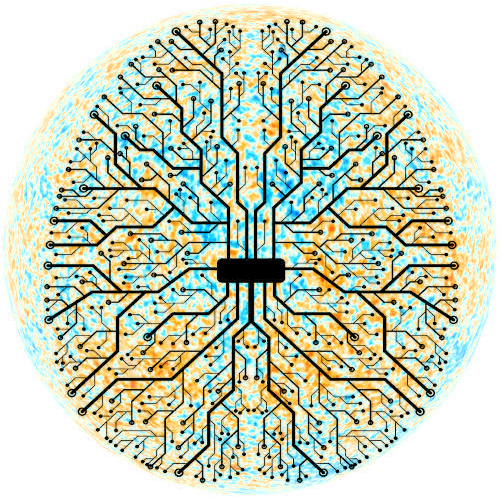
\includegraphics[height=1.0cm]{Ca_Foscari Beamer/handley-lab.png}
%\hspace{0.641\textwidth}{\color{cflink} {\small www.unive.it}} %per 16:9
%\hspace{0.551\textwidth}{\color{cflink} {\small www.unive.it}} %per 4::3
\vspace{0.25cm}
{\color{firebrick} \hrule \hrule  }
\textbf{}
}{}
%%-------------------------------------------------------------

%This block of code defines the information to appear in the Title page
%%%
\title[Inference techniques in gravitational-wave science ] %optional
{Nested sampling for next generation gravitational-wave inference \\ \vspace{0.5em}
}
\author[Metha Prathaban] % (optional)
{Metha Prathaban} %\break %\vfill
\includegraphics[width=0.16\textwidth]{Ca_Foscari Beamer/qr-code.png}}
\date{}



\setbeamertemplate{frametitle}[default][right, rightskip=.5cm] {}
\addtobeamertemplate{frametitle}{\vspace*{-1.4cm}}{}
\setbeamertemplate{navigation symbols}{}
%End of title page configuration block
%------------------------------------------------------------


%------------------------------------------------------------
%The next block of commands puts the table of contents at the 
%beginning of each section and highlights the current section:

\AtBeginSection[]
{
  \begin{frame}
    \frametitle{Table of Contents}
    \tableofcontents[currentsection]
  \end{frame}
}
%------------------------------------------------------------

\begin{document}

%The next statement creates the title page.
\frame{\titlepage}
%---------------------------------------------------------
%This block of code is for the table of contents after
%the title page
% \begin{frame}
% \frametitle{About Me}
% \begin{itemize}
%     \item 3rd year PhD student
%     \item Work on Bayesian numerical method development in context of GWs
% \end{itemize}
% \vspace{2em}
% \bblock{\begin{center}
% Current work is in collaboration with Will Handley and Harry Bevins.
% \end{center}}
% \begin{center}
% 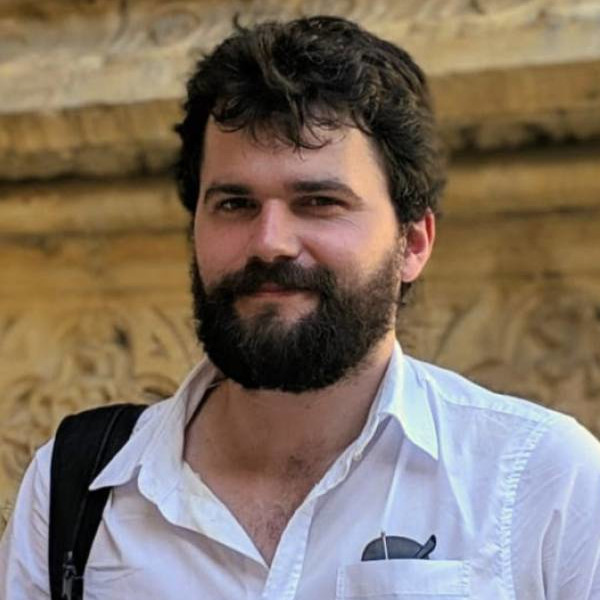
\includegraphics[height=2.0cm]{Ca_Foscari Beamer/will_handley.jpg}
% 
\includegraphics[height=2.0cm]{Ca_Foscari Beamer/harry_bevins.jpg}
% \end{center}
% \eblock
% \end{frame}
%This block of code is for the table of contents after
%the title page
\begin{frame}
\frametitle{Table of Contents}
\tableofcontents
\end{frame}
%---------------------------------------------------------

\begin{frame}
\frametitle{About Me}
\vfill
\begin{itemize}
    \item 3rd year PhD student in Will Handley's group
    \item Handley group works on Bayesian statistical inference and artificial intelligence methodologies, with a focus on analyzing complex datasets from next-generation surveys to explore a wide range of physics questions related to dark matter, dark energy, and the early Universe.
    \item My work on Bayesian numerical method development in context of GWs
\end{itemize} 
\vspace{1em}
\bblock{\begin{center}
The Handley group!
\end{center}}
\begin{center}
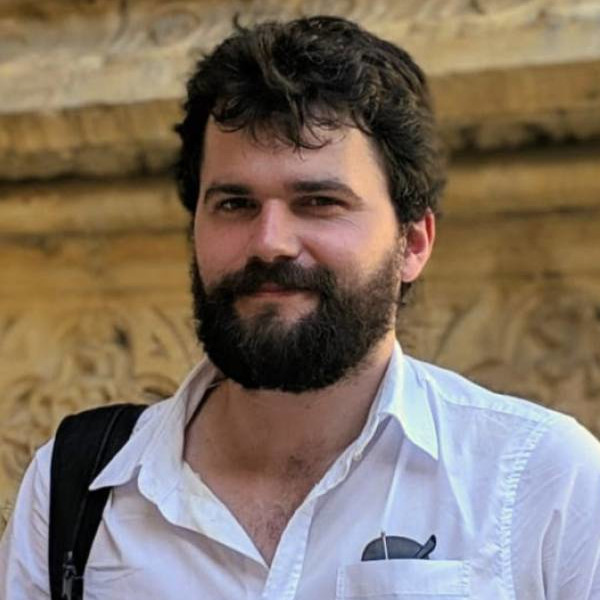
\includegraphics[height=1.0cm]{Ca_Foscari Beamer/will_handley.jpg}
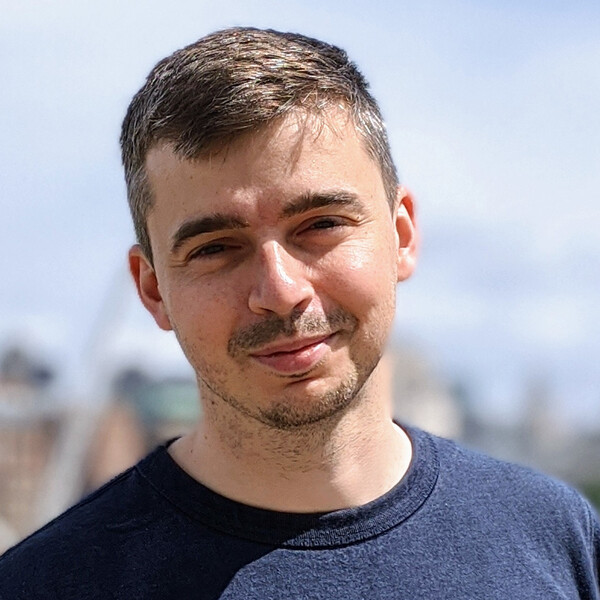
\includegraphics[height=1.0cm]{Ca_Foscari Beamer/david_yallup.jpg}

\includegraphics[height=1.0cm]{Ca_Foscari Beamer/harry_bevins.jpg}
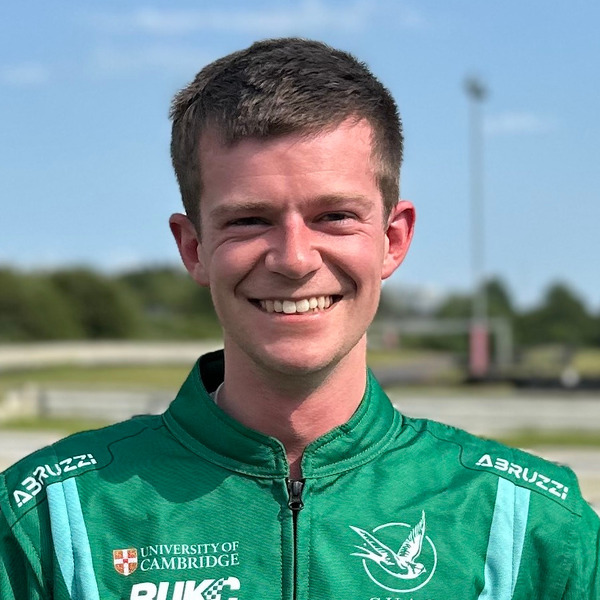
\includegraphics[height=1.0cm]{Ca_Foscari Beamer/adam_ormondroyd.jpg}
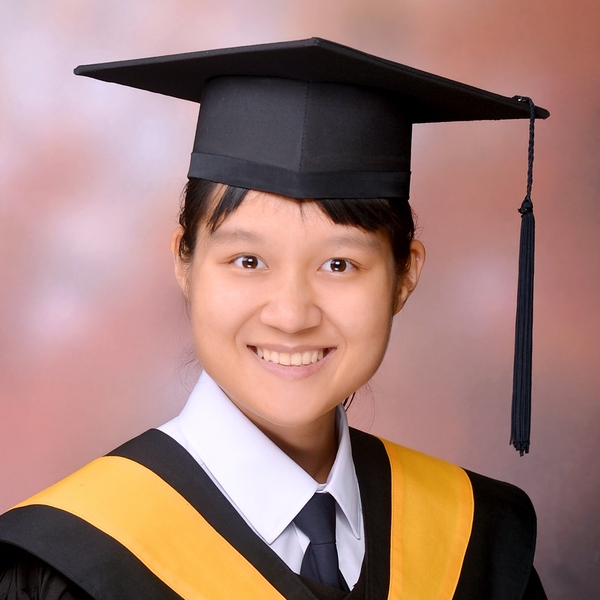
\includegraphics[height=1.0cm]{Ca_Foscari Beamer/wei-ning_deng.jpg}
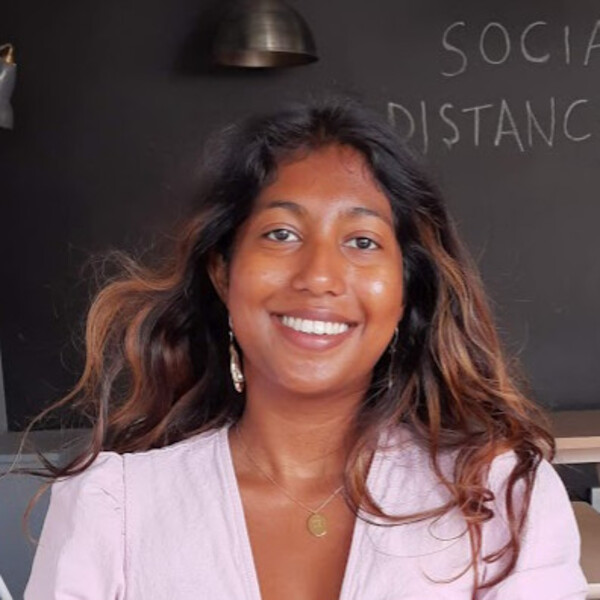
\includegraphics[height=1.0cm]{Ca_Foscari Beamer/metha_prathaban.jpg}
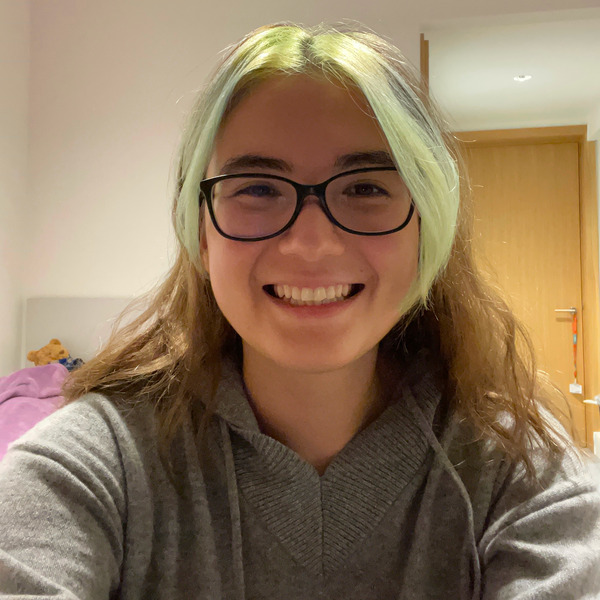
\includegraphics[height=1.0cm]{Ca_Foscari Beamer/sinah_legner.jpg}
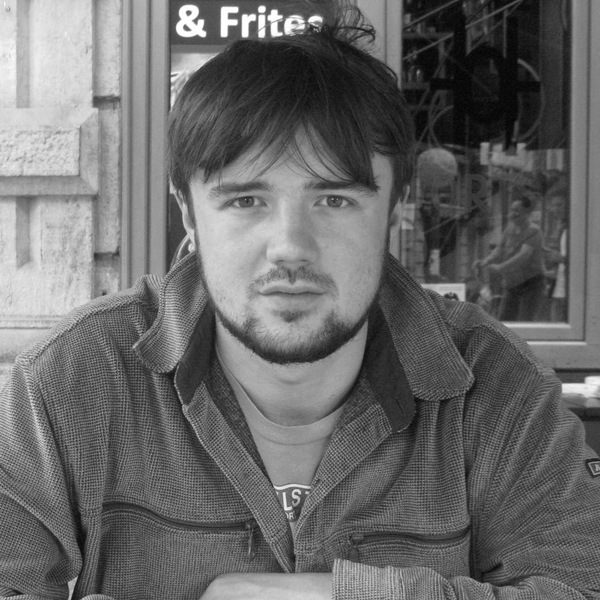
\includegraphics[height=1.0cm]{Ca_Foscari Beamer/sam_leeney.jpg}
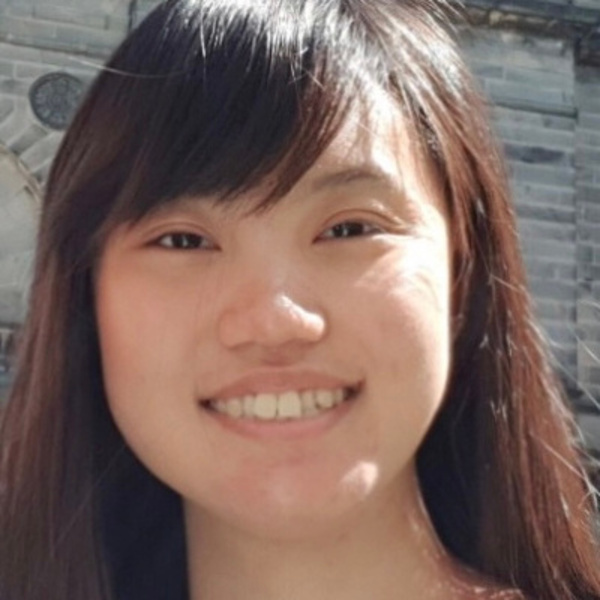
\includegraphics[height=1.0cm]{Ca_Foscari Beamer/dily_ong.jpg}
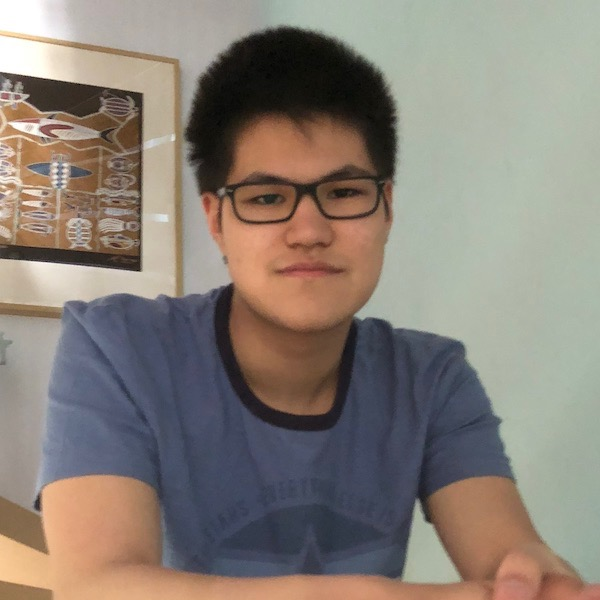
\includegraphics[height=1.0cm]{Ca_Foscari Beamer/namu_kroupa.jpg}
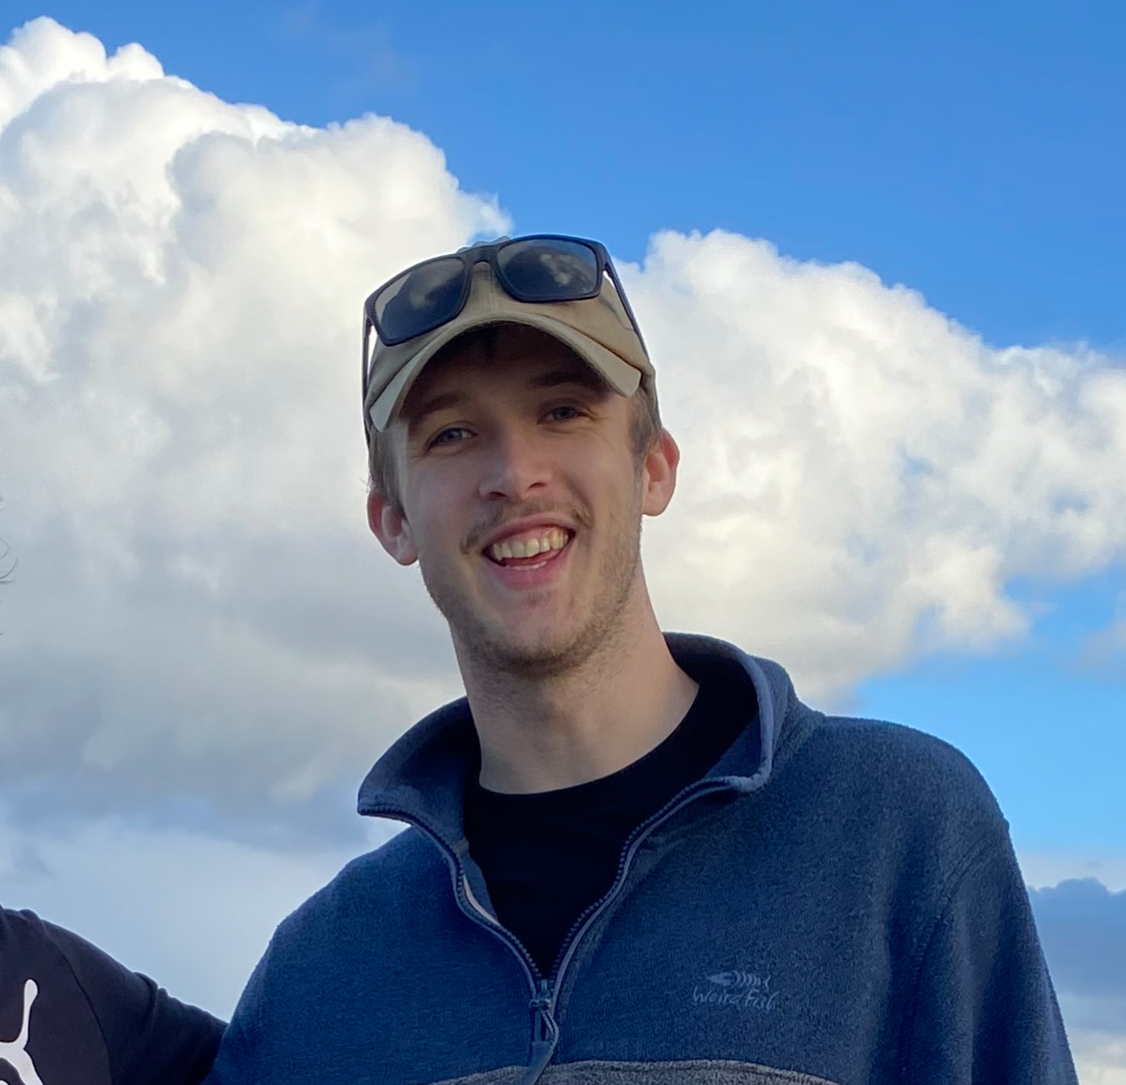
\includegraphics[height=1.0cm]{Ca_Foscari Beamer/toby.png}
\end{center}
\begin{center}
   + others!
\end{center}
\eblock
\end{frame}



\section{Background and context}

\begin{frame}{Inverse problems in GW physics}\vfill

    \begin{tikzpicture}[node distance=5cm, auto]
    % Nodes
    \node (params) [draw, rectangle, rounded corners, minimum width=3cm, minimum height=1cm, align=center] {model parameters \\ \textcolor{cfred}{$\boldsymbol{\theta = \mathcal{M}}\boldsymbol{,q, d_L, t_c ...}$}};
    
    \node (model) [draw, rectangle, minimum width=3cm, minimum height=2cm, align=center, right of=params] {waveform \textcolor{red}{model}};
    
    \node (data) [draw, rectangle, rounded corners, minimum width=3cm, minimum height=1cm, align=center, right of=model] {template for strain waveform \\ 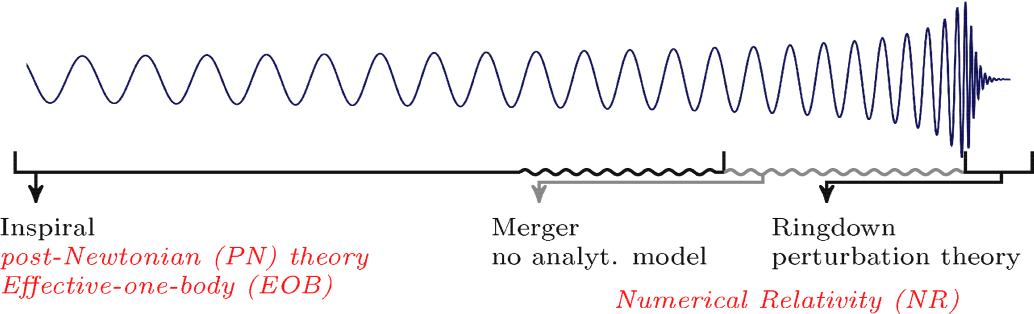
\includegraphics[width=4.2cm]{Ca_Foscari Beamer/waveform_model_inverse.png}};

     % Straight arrow with customizable height and centered text
    \draw[->, thick] 
    ([yshift=0cm] params.east) -- ([yshift=0cm] model.west);
    
    \draw[->, thick] 
    ([yshift=0cm] model.east) -- ([yshift=0cm] data.west);

      % Text above the second rectangle
    \node at ([yshift=0.3cm] model.north) {\textbf{Forward problem}};
    % \draw[->, thick] 
    % ([yshift=-0.2cm] data.west) -- node[midway, below] {\textcolor{cfred}{Inverse problem}} ([yshift=-0.2cm] model.east);

    \node (params2) [draw, rectangle, rounded corners, minimum width=3cm, minimum height=1cm, align=center, below of=params, yshift=2cm] {model parameters, inferred \\ \textcolor{cfred}{$\boldsymbol{\theta}_{\text{est}}$}};
    
    \node (model2) [draw, rectangle, minimum width=3cm, minimum height=2cm, align=center, below of=model, yshift=2cm] {\textcolor{red}{inference}};

    \node (data2) [draw, rectangle, rounded corners, minimum width=3cm, minimum height=1cm, align=center, below of=data, yshift=2cm] {observed signal strain \\ 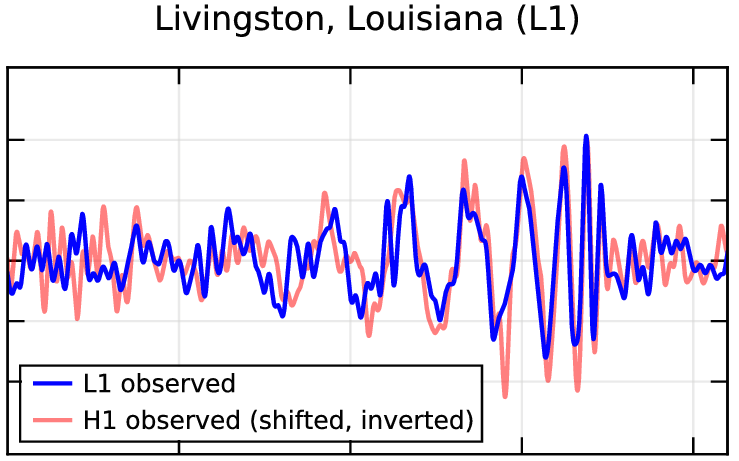
\includegraphics[width=3.5cm]{Ca_Foscari Beamer/gw_example.png.png}};

      % Text above the second rectangle
    \node at ([yshift=0.3cm] model2.north) {\textbf{Inverse problem}};

     % Straight arrow with customizable height and centered text
    \draw[->, thick, line width=1.0mm] 
    ([yshift=0cm] params.east) -- ([yshift=0cm] model.west);
    
    \draw[->, thick, line width=1.0mm] 
    ([yshift=0cm] model.east) -- ([yshift=0cm] data.west);

     % Straight arrow with customizable height and centered text
    \draw[->, thick, line width=1.0mm] 
    ([yshift=0cm] model2.west) -- ([yshift=0cm] params2.east);
    
    \draw[->, thick, line width=1.0mm] 
    ([yshift=0cm] data2.west) -- ([yshift=0cm] model2.east);


    % % Not equal signs (≠) between vertical pairs of rectangles (ensure correct syntax for \visible)
    %\visible<1>{\node at (data -| data2) [yshift=-1.4cm] {\textcolor{red}{$\boldsymbol{\neq}$ (observational error)}};}
    %\visible<1>{\node at (params -| params2) [yshift=-1.4cm] {\textcolor{red}{$\boldsymbol{\neq}$ (error propagation)}};}
    
\end{tikzpicture}

\end{frame}

%Changing visibility of the text
\begin{frame}{Bayes' Theorem}

Given some model $\mathcal{M}$ and observed signal $\mathcal{D}$, Bayes' theorem enables us to relate the \textcolor{RoyalBlue}{posterior} probability of the set of parameters $\theta$ which generated the signal to the \textcolor{Purple}{likelihood} of the $\mathcal{D}$ given $\theta$ and the \textcolor{BurntOrange}{prior} probability of $\theta$ given $\mathcal{M}$:
\vfill
\begin{equation}
    \textcolor{RoyalBlue}{\mathcal{P}(\theta | D, \mathcal{M})} = \frac{\textcolor{Purple}{P(D | \theta, \mathcal{M})} \textcolor{BurntOrange}{P(\theta | \mathcal{M})}}{\textcolor{red}{P(D | \mathcal{M})}} = \frac{\textcolor{Purple}{\mathcal{L}(D | \theta)} \textcolor{BurntOrange}{\pi(\theta)}}{\textcolor{red}{\mathcal{Z}}}
\end{equation}
\vfill
The \textcolor{red}{evidence}, \textcolor{red}{$\mathcal{Z}$}, plays a key role in model comparison.
\end{frame}

\begin{frame}{Bayesian inference}
\begin{columns}
    
\column{0.5\textwidth}
\begin{itemize}
    \item Define \textcolor{BurntOrange}{prior}, \textbf{sample} (unnormalized) \textcolor{RoyalBlue}{posterior} ($\mathcal{L}(\textbf{d} | \theta) \times \pi(\theta)$).
    % \item Cannot plot full posterior distribution but can plot 1D and 2D \textbf{marginal} distributions (e.g. $\mathcal{P}(\mathcal{M}, q, \chi_\text{eff} | D)$) by integrating over all other parameters.
\end{itemize}
\vspace{2em}
\raggedright
Challenges:\vfill
    \begin{itemize}
        \item High-dimensional parameter spaces $\Rightarrow$ \textcolor{RoyalBlue}{posterior} occupies vanishingly small region of \textcolor{BurntOrange}{prior}.
        \item Complex waveform models with high costs
    \end{itemize}
    \vfill 

\column{0.5\textwidth}\
\vspace{-2em}
\centering
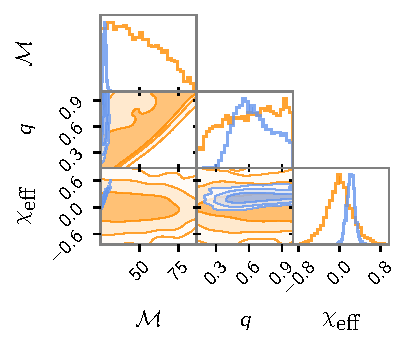
\includegraphics[]{Ca_Foscari Beamer/presentation_triangleplot.pdf}
\end{columns}
\end{frame}

\begin{frame}{Samplers}\vfill
Goal is efficient exploration of parameter space, to do GW inference in feasible timescales. 
\vfill  
    \textcolor{RoyalBlue}{Posterior} samplers:
    \begin{itemize}
        \item Metropolis-Hastings 
        \item Hamiltonian Monte-Carlo
        \item Ensemble samplers
    \end{itemize}
    \vfill
    None of these calculate the \textcolor{red}{evidence}, \textcolor{red}{$\mathcal{Z}$} - crucial for Bayesian model comparison (e.g. testing for precession vs. no precession)!  
\end{frame}

%Example of the \pause command
\begin{frame}
\frametitle{Nested sampling (NS)}\vfill
Nested sampling first and foremost calculates \textcolor{red}{evidence}, $\textcolor{red}{\mathcal{Z}} = \int \mathcal{L(\theta)} \pi(\theta) d\theta$.
\begin{minipage}[]{0.35\textwidth}
\vspace{20em}
\visible<1>{
\begin{tikzpicture}
\def\svgwidth{\textwidth}
\input{NS_cartoon_2.pdf_tex}
\end{tikzpicture}
}
\visible<2>{
\begin{tikzpicture}
\def\svgwidth{\textwidth}
\hspace{-0.39cm}
\input{NS_cartoon_3.pdf_tex}
\end{tikzpicture}
}
\visible<3>{
\begin{tikzpicture}
\def\svgwidth{\textwidth}
\hspace{-0.78cm}
\input{NS_cartoon_4.pdf_tex}
\end{tikzpicture}
}
\visible<4>{
\begin{tikzpicture}
\def\svgwidth{\textwidth}
\hspace{-1.2cm}
\input{NS_cartoon_5.pdf_tex}
\end{tikzpicture}
}
\visible<5>{
\begin{tikzpicture}
\def\svgwidth{\textwidth}
\hspace{-1.6cm}
\input{NS_cartoon_5.pdf_tex}
\end{tikzpicture}
}
\vspace{-5em}
\end{minipage}\hfill
\begin{minipage}{0.5\textwidth}
    \begin{itemize}
        \item<1-> Prior is populated with set of `live points'.
        \item<2-> At each iteration $i$, point is lowest likelihood is deleted and new live point is drawn, which must have a likelihood higher than that of the deleted point.
        \item<4-> Live points compress exponentially towards peak of likelihood.
        \item<5-> \textcolor{red}{Evidence} is calculated as weighted sum over deleted (`dead') points.
    \end{itemize}
    %\vspace{-2.5em}
\end{minipage}
\end{frame}

\begin{frame}{Runtime of NS}
Time of convergence of NS: {\tiny 2212.01760}
\vfill
    \begin{equation}
        T \propto \tikzmarknode{a1}{T_{\mathcal{L}}} \times \tikzmarknode{a2}{f_{\textrm{sampler}}} \times \tikzmarknode{a3}{D_{\textrm{KL}}} \times \tikzmarknode{a4}{n_{\textrm{live}}} 
    \end{equation}
    \begin{tikzpicture}[remember picture, overlay]
    \visible<2->{\draw[explain, <-, thick, firebrick](a4)--++(1.5,1)node[above]{resolution};}
    \visible<1->{\draw[explain, <-, thick, firebrick](a1)--++(-2,1)node[above]{likelihood evaluation time};}
    \visible<3->{\draw[explain, <-, thick, firebrick](a2)--++(-2.8,-1.7)node[below]{drawing new live point};}

    \onslide<3->{\node[anchor=south, inner sep=12pt] at (current page.south west) {\hspace{8em}
            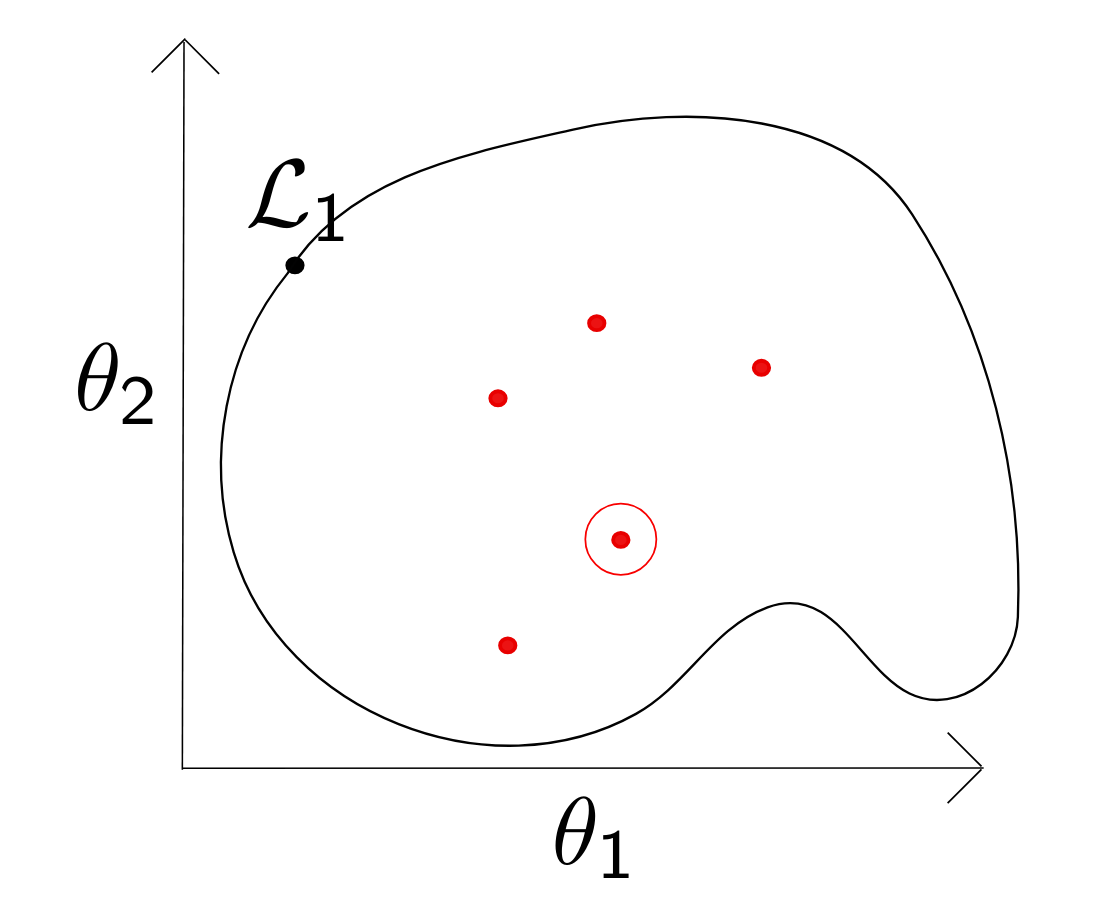
\includegraphics[width=0.2\textwidth]{Ca_Foscari Beamer/Screenshot from 2024-11-22 10-06-12.png}
        };}

    \onslide<4->{\node[anchor=south, inner sep=15pt] at (current page.south east) {\hspace{-8em}
        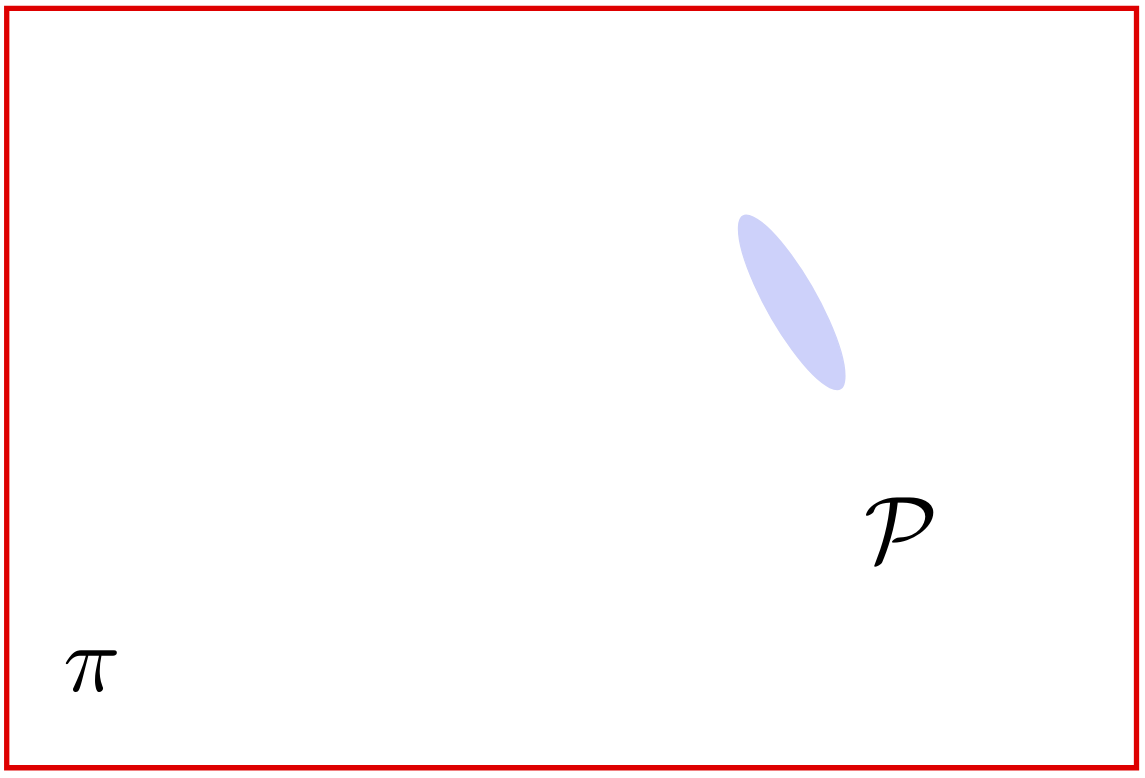
\includegraphics[width=0.17\textwidth]{Ca_Foscari Beamer/kl_div_screenshot.png}
    };}
        
    \visible<4->{\draw[explain, <-, thick, firebrick](a3)--++(1.2,-0.6)node[below]{compression from \textcolor{BurntOrange}{prior} to \textcolor{RoyalBlue}{posterior} ($\approx \mathrm{ln}\frac{V_\pi}{V_\mathcal{P}}$)};}
    \end{tikzpicture}
\end{frame}



\begin{frame}{Current vs. future data}
 \begin{minipage}{0.47\textwidth} \vspace{0.5cm}
 \bblock{\centering LVK data so far}
\begin{itemize} 
\item Short-duration signals from compact binary coalescences (CBCs)
\item End of O4a: $\approx 200$ confident detections 
\item Detection rate: $\approx 1$ every few days 
    \begin{itemize}
        \item Signals not overlapping
    \end{itemize}
\item BBH mergers last seconds, BNS mergers last minutes
\item Computationally intensive to analyse, but doable with current pipelines.
\end{itemize} 
\eblock
\end{minipage}\hfill                                        \begin{minipage}{0.47\textwidth}\vspace{0.6cm}                        \centering                                          
    \bblock{\centering ET + CE}
    \begin{itemize}
        \item Ten-fold improvement in sensitivity compared to 2G detectors
        \item Detection rate: $\approx 10^5-10^6$ BBH and $\approx 7 \times 10^4$ BNS mergers per year
        \item Wider frequency band $\Rightarrow$ more intermediate mass BHs
        \item Improved localization
        \item Significantly higher SNR
        \item Longer signal durations %talk about noise
        \begin{itemize}
            \item Overlapping signals expected
        \end{itemize}
        \item New GW sources
    \end{itemize}
    \eblock
\end{minipage}                                                    
\end{frame}

\begin{frame}{Scaling of traditional methods}
    \begin{equation}
        T_{\textrm{total}} \propto \tikzmarknode{N}{N_{\textrm{signals}}} \times \tikzmarknode{Tl}{T_{\mathcal{L}}} \times \tikzmarknode{a2}{f_{\textrm{sampler}}} \times  \tikzmarknode{DKL}{D_{\textrm{KL}}} \times \tikzmarknode{a4}{n_{\textrm{live}}} 
    \end{equation}

\begin{tikzpicture}[remember picture, overlay]
\visible<1->{\draw[explain, <-, thick, firebrick] (N)--++(-1,-1) 
    node[below]{higher sensitivity};}
    
\visible<2->{\draw[explain, <-, thick, firebrick] (DKL)--++(0.9,-0.7) 
    node[below]{higher SNR + longer signal $\Rightarrow$ narrower posterior};}

    \visible<3->{\draw[explain, <-, thick, firebrick] (Tl)--++(-2,1) 
    node[above]{longer signal duration $\Rightarrow$ slower waveform generation};}

    \visible<4->{\node (text) at (10.05, -0.8) {\textcolor{firebrick}{overlapping signals $\Rightarrow$ joint PE}};}


    \visible<5->{\node (L) at (3.75, 2.6) {\textcolor{firebrick}{overlapping signals $\Rightarrow$ joint likelihood}};}

    \visible<6->{\node (text2) at (10.55, -1.4) {\textcolor{firebrick}{duration $\gtrsim 10 \textrm{mins} \Rightarrow$ extra modeling}};} %earth's rotation, varying PSD

    \visible<7->{\node (text4) at (10.5, -2) {\textcolor{firebrick}{non-stationary noise}};}
    \visible<7->{\node (L) at (3.75, 3.1) {\textcolor{firebrick}{non-stationary noise}};}
    \visible<8->{\node (text3) at (7, -3) {\textbf{Billions to quadrillions of CPU core hours for 1 month of ET data...} \tiny 2412.02651};} %cite John Veitch

    
\end{tikzpicture}
\end{frame}

\begin{frame}{Established acceleration attempts}
\vfill
    \visible<1->{\begin{block}{Heterodyning}
        Exploits the smooth changes in GW waveforms near the maximum likelihood point. Assigns fiducial source parameter close to the true value and uses coarser frequency resolution. 
    \end{block}
    \begin{block}{Reduced Order Quadrature}
        Approximates the waveform model as a linear combination of a small number of pre-trained bases evaluated at representative frequencies. 
    \end{block}
    \begin{block}{Multibanding}
        Adjusts data resolution for gravitational wave signals across frequency bands, particularly during low-frequency early inspiral stage of CBCs. 
    \end{block}} \vfill
    \centering
    \visible<2->{\textbf{Even with these, millions of CPU core hours for 1 month of ET data.} \tiny 2412.02651}
\end{frame}

\setbeamertemplate{footline}{%
  \leavevmode%
  \hbox to \paperwidth{%
    % First box (Email address) - Exactly 1/3 of paperwidth
    \begingroup
    \setlength{\fboxsep}{2pt}% Padding inside the box
    \colorbox{firebrick}{\makebox[\dimexpr0.333\paperwidth\relax][c]{\strut\textcolor{white}{\texttt{myp23@cam.ac.uk}}}}%
    \endgroup
    % Second box (Custom text) - Exactly 1/3 of paperwidth
    \begingroup
    \setlength{\fboxsep}{2pt}% Padding inside the box
    \colorbox{firebrick}{\makebox[\dimexpr0.333\paperwidth\relax][c]{\strut\textcolor{white}{https://arxiv.org/abs/2411.17663}}}%
    \endgroup
    % Third box (Frame number) - Exactly 1/3 of paperwidth
    \begingroup
    \setlength{\fboxsep}{2pt}% Padding inside the box
    \colorbox{firebrick}{\makebox[\dimexpr0.334\paperwidth\relax][c]{\strut\textcolor{white}{\insertframenumber/\inserttotalframenumber}}}%
    \endgroup
  }%
  \vskip0pt%
}

\section{Accelerating NS with ML}

\setbeamertemplate{headline}{
    \vspace{0.25cm} \ \ 
    
\includegraphics[height=1.0cm]{Ca_Foscari Beamer/cambridge-cropped.pdf}
    
\includegraphics[height=1.0cm]{kicc.png}
    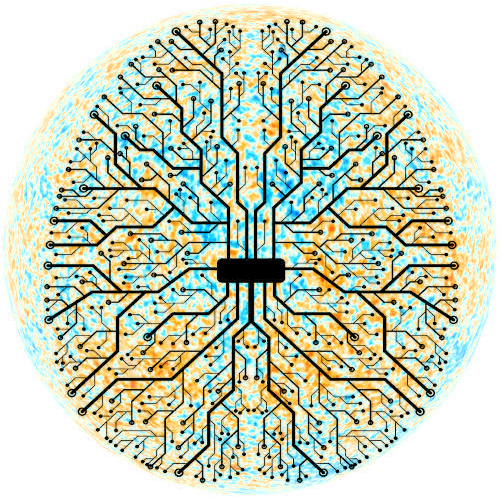
\includegraphics[height=1.0cm]{Ca_Foscari Beamer/handley-lab.png}
    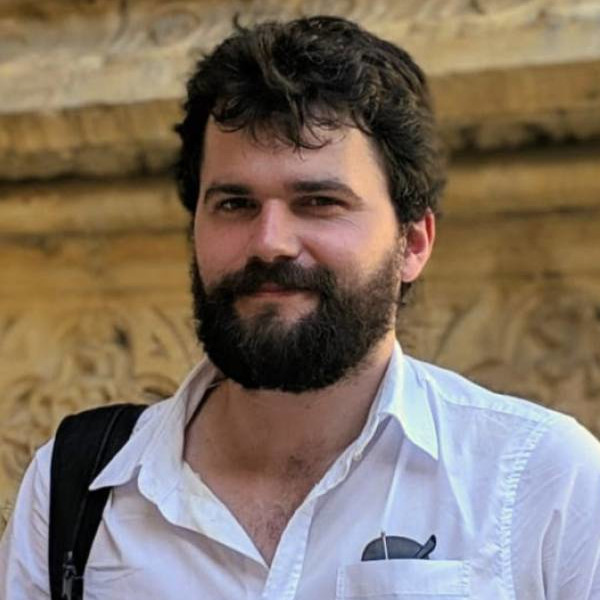
\includegraphics[height=1.0cm]{Ca_Foscari Beamer/will_handley.jpg} % Unique to this slide
    
\includegraphics[height=1.0cm]{Ca_Foscari Beamer/harry_bevins.jpg}
    \vspace{0.25cm}
    {\color{firebrick} \hrule \hrule}
  }

  
\begin{frame}{ML for traditional methods}


        \begin{equation}
        T \propto \tikzmarknode{a1}{T_{\mathcal{L}}} \times \tikzmarknode{a2}{f_{\textrm{sampler}}} \times 
        \onslide<4->{\tikz\node[draw=firebrick, inner sep=8.5pt, circle, overlay, shift={(10pt,2pt)}]{}} 
        \tikzmarknode{a3}{D_{\textrm{KL}}} \times \tikzmarknode{a4}{n_{\textrm{live}}} 
    \end{equation}
    \begin{tikzpicture}[remember picture, overlay]
    % \visible<2->{\draw[explain, <-, thick, firebrick](a4)--++(1.5,1)node[above]{resolution};}
    \visible<1->{\draw[explain, <-, thick, firebrick](a1)--++(-2,1)node[above]{ROM, surrogates};} % artificial neural networks to map gravitational-wave source parameters into basis coefficients
    \visible<2->{\draw[explain, <-, thick, firebrick](a2)--++(-2.8,-1.7)node[below]{\textsc{nessai}};}

    \onslide<2->{\node[anchor=south, inner sep=12pt] at (current page.south west) {\hspace{8em}
            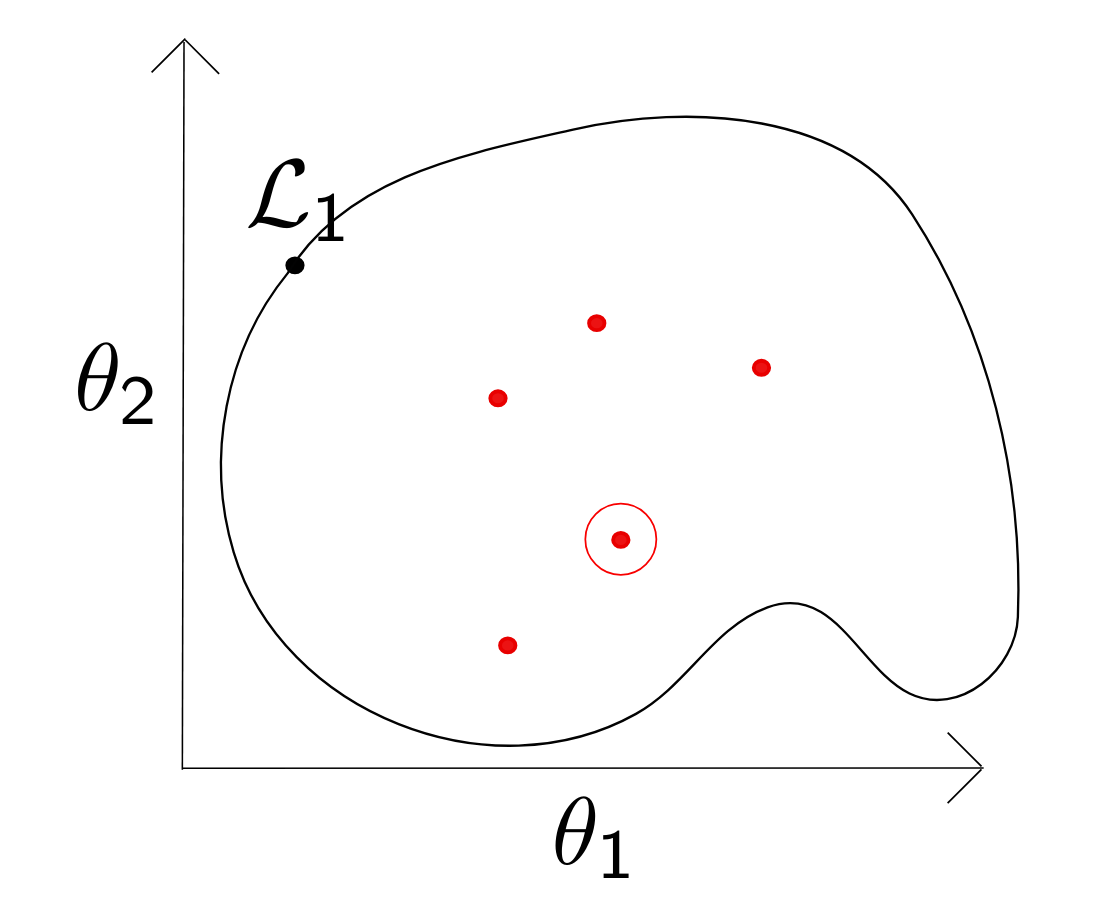
\includegraphics[width=0.2\textwidth]{Ca_Foscari Beamer/Screenshot from 2024-11-22 10-06-12.png}
        };}

    \onslide<3->{\node[anchor=south, inner sep=15pt] at (current page.south east) {\hspace{-8em}
        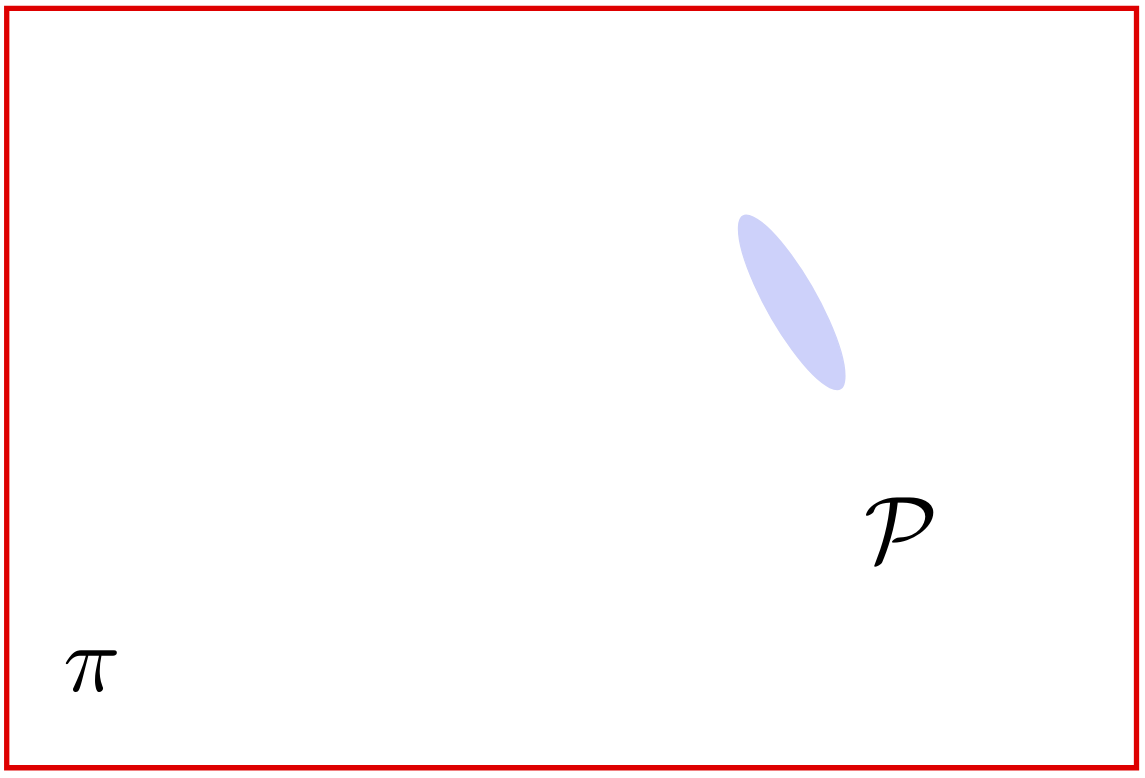
\includegraphics[width=0.17\textwidth]{Ca_Foscari Beamer/kl_div_screenshot.png}
    };}
    \visible<3>{\draw[explain, <-, thick, firebrick](a3)--++(1.2,-0.6)node[below]{not as baked-in as you might think!};}
    \visible<4->{\draw[explain, <-, thick, firebrick](a3)--++(1.2,-0.6)node[below]{focus of this section};}
    \end{tikzpicture}
    % Have only just begun to set benchmarks for acceleration methods for 3G era - lots more to be done here to study the speedups we can expect.
\end{frame}

\begin{frame}{Uncertainty of NS}

\begin{block}{Time of convergence of NS}
    \begin{equation}
        T \propto T_{\mathcal{L}} \times f_{\textrm{sampler}} \times D_{\textrm{KL}} \times n_{\textrm{live}} 
    \end{equation}
\end{block}
\begin{block}{Uncertainty in log$\textcolor{red}{\mathcal{Z}}$}
    \begin{equation}
        \sigma \propto \sqrt{D_{\textrm{KL}} / n_{\textrm{live}}}
    \end{equation}
\end{block}

\alert{Precision-normalized} runtime has quadratic dependence on KL divergence. \textcolor{cfgrey}{2212.01760}
    
\end{frame}

\begin{frame}{REACH}
\vspace{2em}
One way to do this (REACH):
\vfill
\centering
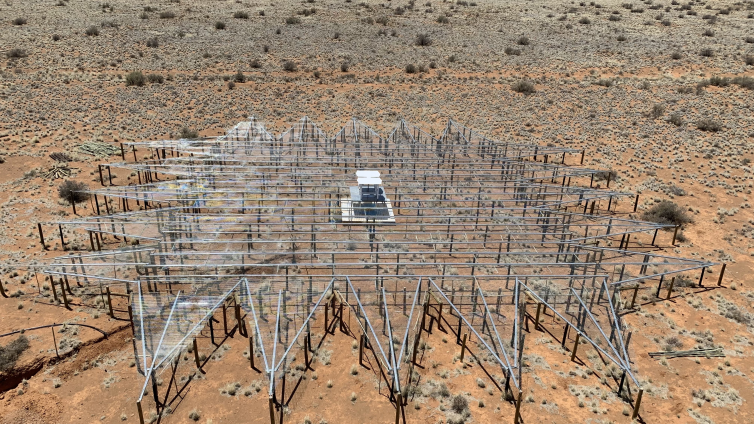
\includegraphics[width=0.6\textwidth]{Ca_Foscari Beamer/antenna.png}

\end{frame}

\begin{frame}{Reducing $D_{\textrm{KL}}$}
\vspace{3.5em}
One way to do this (REACH):

\begin{minipage}[]{0.45\textwidth}\vspace{22em}
%\includegraphics<1>[0.9\textwidth]{Ca_Foscari Beamer/antenna.png}%
\visible<1>{
\begin{tikzpicture}
\def\svgwidth{0.9\textwidth}
\input{PR_cartoon.pdf_tex}
\end{tikzpicture}
}
\visible<2>{
\begin{tikzpicture}
\def\svgwidth{0.9\textwidth}
\hspace{-0.96em}
\input{PR_cartoon_2.pdf_tex}
\end{tikzpicture}
}
\visible<3>{
\begin{tikzpicture}
\def\svgwidth{0.9\textwidth}
\hspace{-2em}
\input{PR_cartoon_3.pdf_tex}
\end{tikzpicture}
}
\end{minipage}
\begin{minipage}{0.45\textwidth}\vspace{-8em}
\begin{itemize}
    \item<1-> Perform low resolution (low live points) run first to roughly identify where \textcolor{RoyalBlue}{posterior} lies.
    \item<2-> Then set off second, high resolution, run with \textbf{narrower} box \textcolor{BurntOrange}{prior} (much quicker).
    \item<3-> \textcolor{red}{Evidence} has \textbf{changed} (since different prior), but easy to correct (multiply new evidence by $\frac{V_{\pi^\ast}}{V_\pi}$)
\end{itemize}
\end{minipage}

\end{frame}

\begin{frame}{NFs}
    \begin{itemize}\vspace{3em}

    \item<1-> Can iterate on this by using \textbf{normalizing flows} (NF) to learn the rough \textcolor{RoyalBlue}{posterior}.
    \item<2-> NFs perform density estimation, by learning a series of invertible mappings from the standard normal distribution to the target (posterior). 
\end{itemize}\vspace{0em}
    \visible<2->{\centering 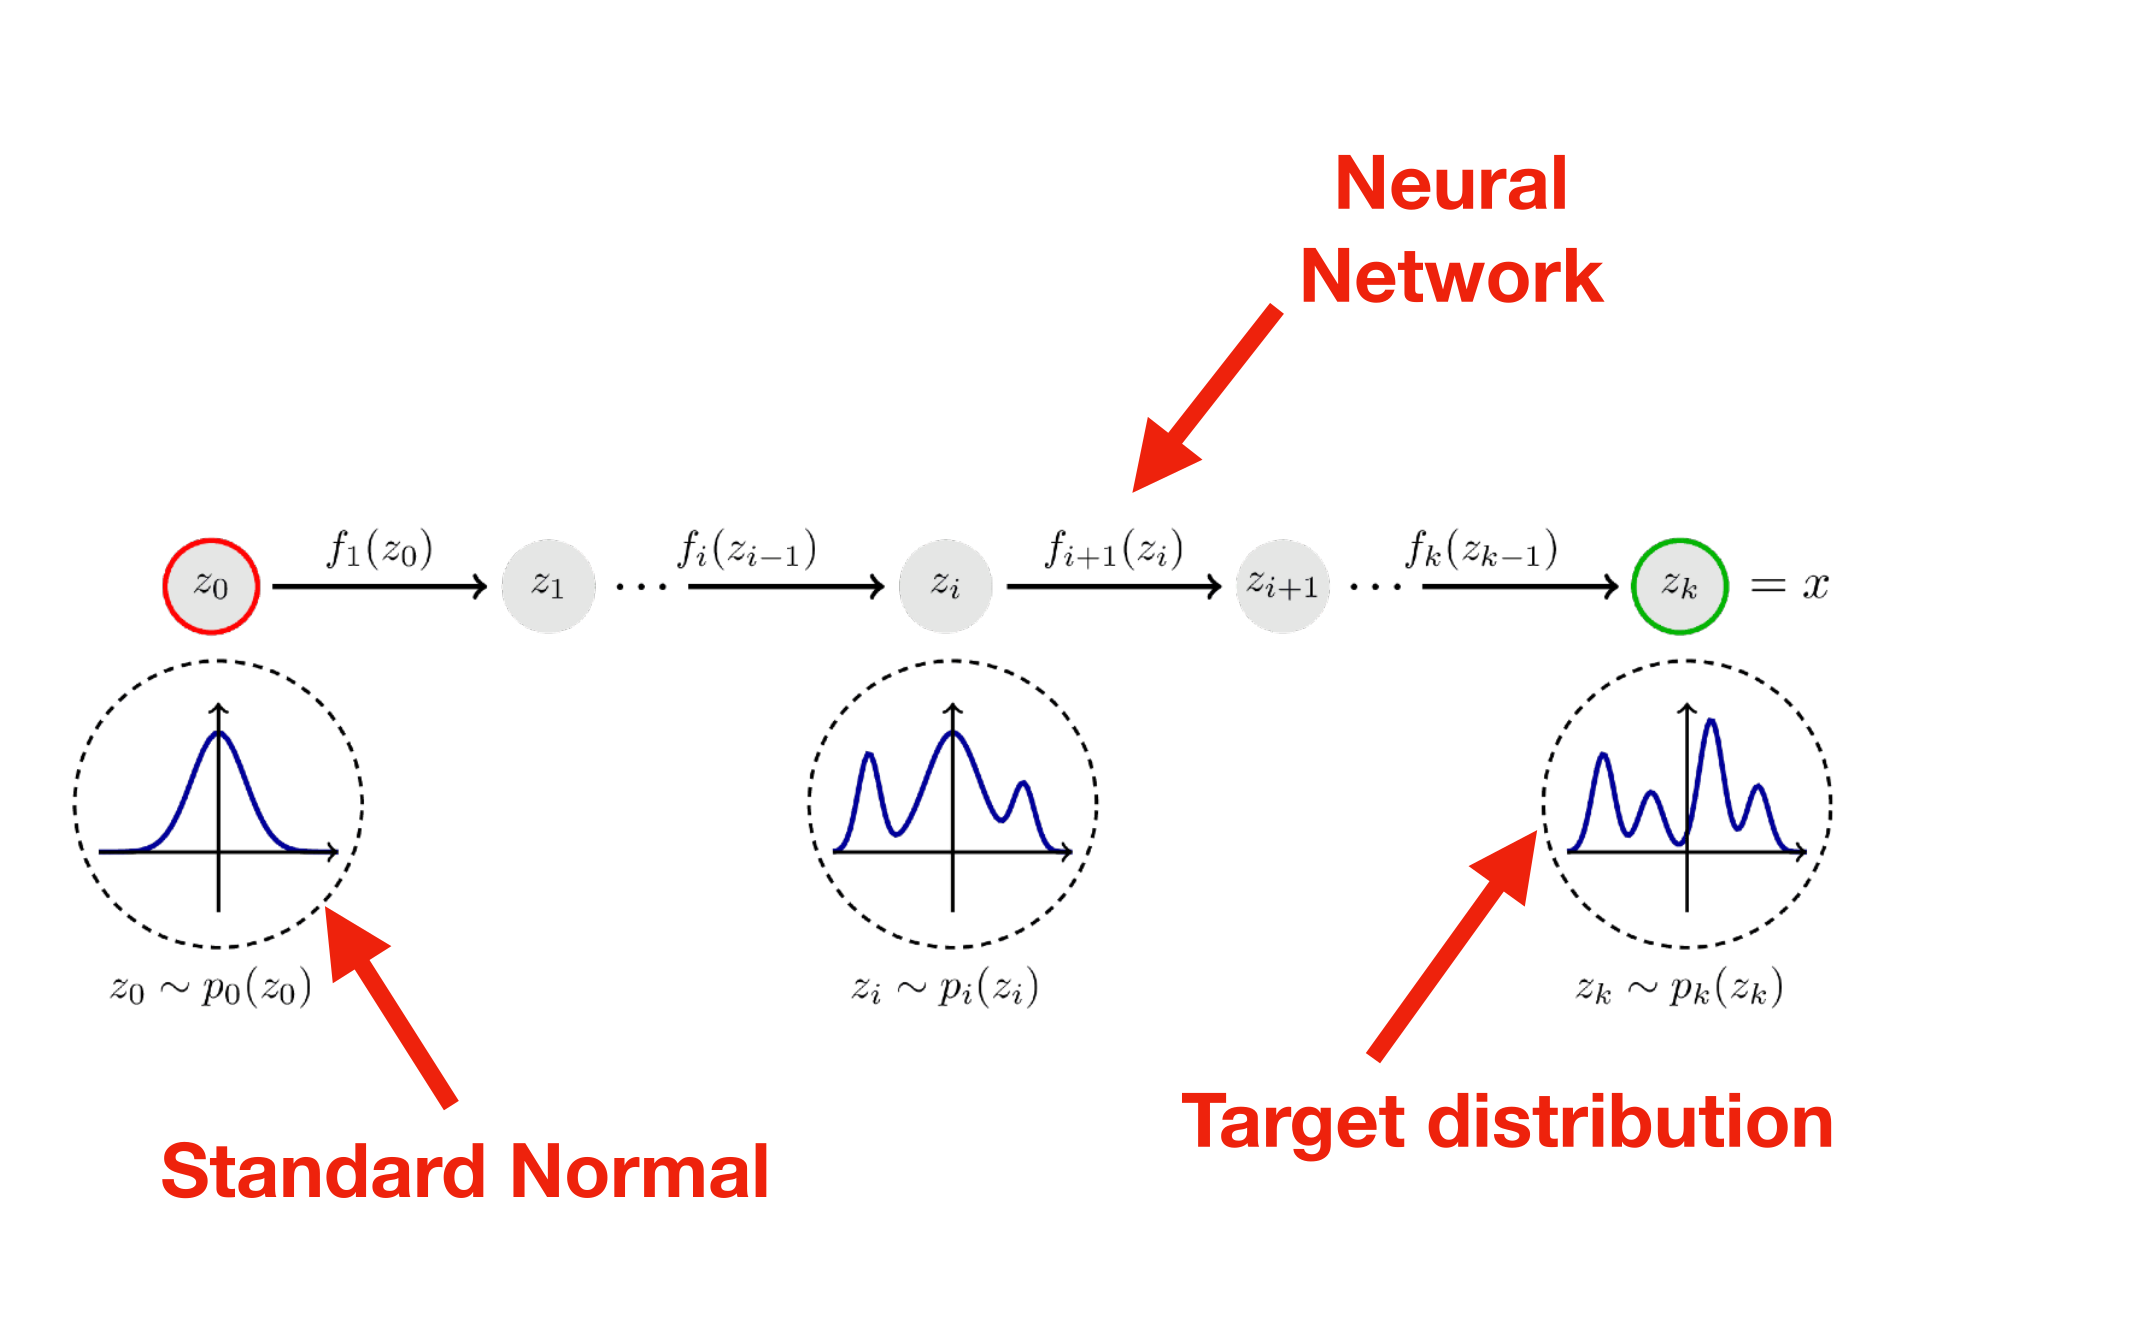
\includegraphics[width=0.5\textwidth]{Ca_Foscari Beamer/NF_diagram.png}}
\end{frame}

\begin{frame}{NF + PR}
\begin{itemize}\vspace{1em}
    \item<1-> Use \textbf{normalizing flows} (NF) to learn the rough \textcolor{RoyalBlue}{posterior}, and use this as our updated prior, $\pi^\ast$.
    \item<1-> In this case, can't do our trick of correcting the second \textcolor{red}{evidence} by volume ratio, $\frac{V_{\pi^\ast}}{V_{\pi}}$!
    \item<1-> Must rely on another technique to get around this!
\end{itemize}\vspace{2em}
\visible<2->{\textcolor{red}{Posterior repartitioning} (PR) can help us with this! (see e.g. \textcolor{cfgrey}{2212.01760})}\hspace{2em}\vfill
\begin{minipage}{1\textwidth}
\visible<2->{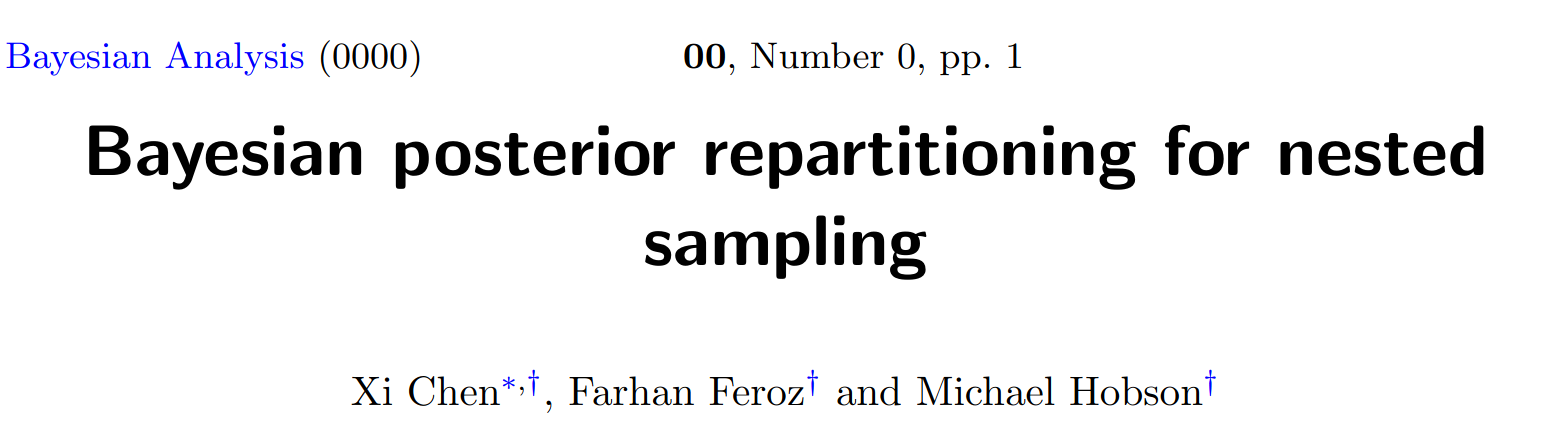
\includegraphics[width=0.3\textwidth]{Ca_Foscari Beamer/PR1.png}
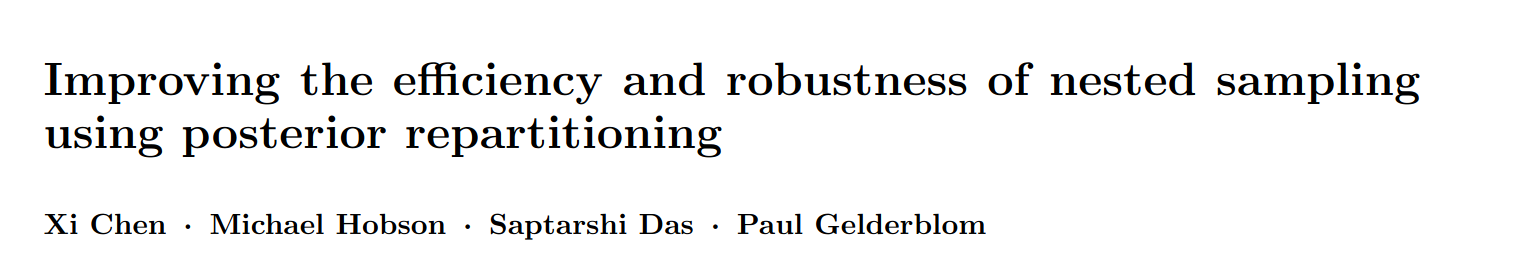
\includegraphics[width=0.38\textwidth]{Ca_Foscari Beamer/PR2.png}
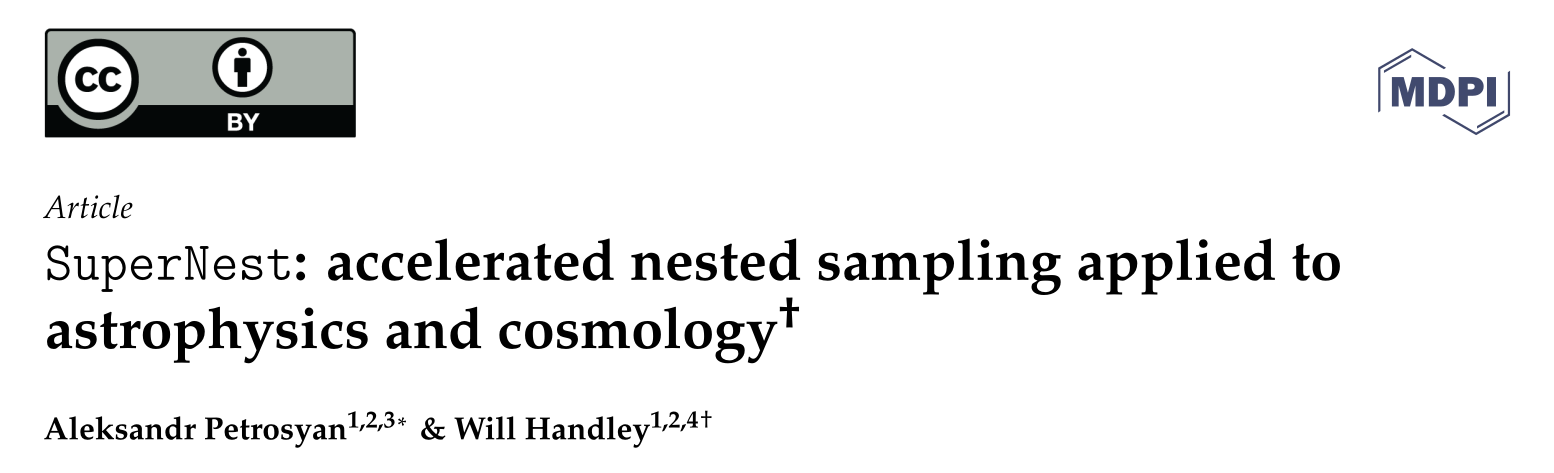
\includegraphics[width=0.3\textwidth]{Ca_Foscari Beamer/PR3.png}
}
\end{minipage}
\end{frame}\begin{frame}{Posterior repartitioning (PR)}\vfill
\begin{itemize}
    \item \textcolor{red}{Evidence} and \textcolor{RoyalBlue}{posterior} only depend on product of $\mathcal{L}$ and $\pi$: \vspace{-2em}
\begin{multicols}{2}
\begin{equation}
    \textcolor{red}{\mathcal{Z}} = \int \textcolor{Purple}{\mathcal{L}(\theta)} \textcolor{BurntOrange}{\pi(\theta)} d\theta
\end{equation}\break
\begin{equation}
    \textcolor{RoyalBlue}{\mathcal{P}(\theta)} = \frac{\textcolor{Purple}{\mathcal{L}(\theta)} \textcolor{BurntOrange}{\pi(\theta)}}{\textcolor{red}{\mathcal{Z}}}
\end{equation}
\end{multicols}

    \bblock{We are free to redefine the likelihood and prior however we like - as long as the product is the same! \textcolor{cfgrey}{arXiv:1908.04655}}
    \centering
    \begin{equation}
        \textcolor{red}{\tilde{\mathcal{Z}}} = \int \textcolor{Purple}{\tilde{\mathcal{L}}(\theta)} \textcolor{BurntOrange}{\tilde{\pi}(\theta)} d\theta = \int \textcolor{Purple}{\mathcal{L}(\theta)} \textcolor{BurntOrange}{\pi(\theta)} d\theta = \textcolor{red}{\mathcal{Z}}
    \end{equation}
\eblock
\end{itemize}

\end{frame}

\begin{frame}{PR (cont.)}
\begin{itemize}

\vfill
     \item Many sampling algorithms do not distinguish between $\textcolor{Purple}{\mathcal{L}}$ and $\textcolor{BurntOrange}{\pi}$ at the algorithmic level.
    \item e.g. Metropolis-Hastings acceptance ratio only depends on the \textbf{joint distribution}, $\textcolor{Purple}{\mathcal{L}(\theta)} \textcolor{BurntOrange}{\pi(\theta)}$.
   \item Nested sampling does distinguish between prior and likelihood at the algorithmic level, by \textcolor{red}{`sampling from the prior $\pi$, subject to the hard likelihood constraint, $\mathcal{L}$'}.
\vfill
\item $\textcolor{red}{\mathcal{Z}}$ and $\textcolor{RoyalBlue}{\mathcal{P}}$ will not change if we repartition \textcolor{Purple}{$\mathcal{L}$} and \textcolor{BurntOrange}{$\pi$}, \textbf{but} $\boldsymbol{\mathcal{D}}_\mathbf{\mathrm{\textbf{KL}}}$ \textbf{will}.
\end{itemize}
\end{frame}

\begin{frame}{PR-NS w/ NFs}
    \centering
    \visible<1->{$\textcolor{BurntOrange}{\pi(\theta)} \longrightarrow \textcolor{BurntOrange}{\text{NF}(\theta)}$ }
    \vfill
    \visible<2->{$\textcolor{Purple}{\mathcal{L}(\theta)} \longrightarrow \textcolor{Purple}{\frac{\mathcal{L}(\theta)\pi(\theta)}{\text{NF}(\theta)}}$}
    \vfill
    \visible<3->{$\mathcal{D}_\mathrm{KL} \approx \text{log}\frac{V_\text{NF}}{V_\mathcal{P}}$}
\end{frame}

\begin{frame}{Demo on simulated example}
\begin{minipage}{0.45\textwidth}\vspace{1em}
\begin{itemize}
    \item<1-> Perform low resolution run on simulated data.
    \item<2-> Train NF on the weighted samples.
    \item<3-> Use this as `repartitioned prior' for new high resolution run (using PR to also update likelihood accordingly to same evidences and posteriors out).
\end{itemize}
\end{minipage}
\begin{minipage}{0.45\textwidth}
        \visible<1>{\vspace{2.5em}\begin{figure}
        \centering
        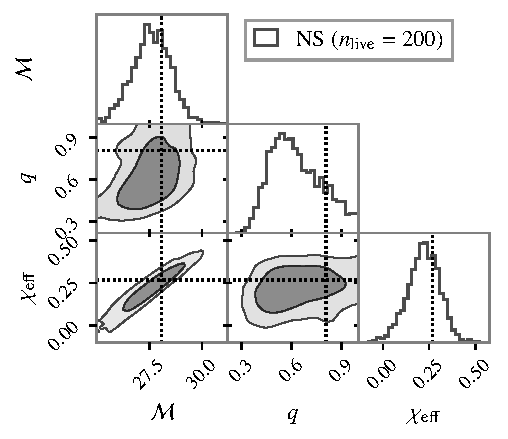
\includegraphics[]{Ca_Foscari Beamer/presentation_simulated_1.pdf}
    \end{figure}}
    \visible<2-3>{\vspace{-18.5em}\begin{figure}
        \centering
        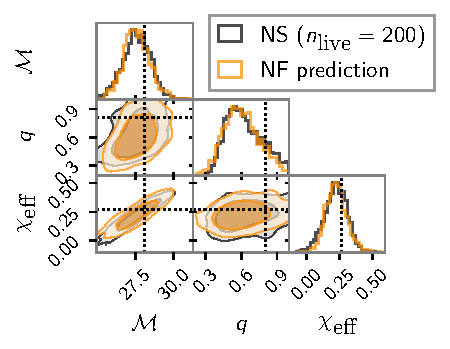
\includegraphics[]{Ca_Foscari Beamer/presentation_simulated_2.pdf}
    \end{figure}}
    \visible<4>{\vspace{-18em}\begin{figure}
        \centering
        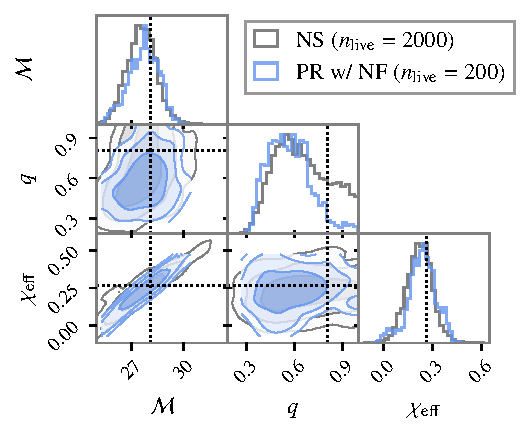
\includegraphics[]{Ca_Foscari Beamer/presentation_simulated_3.pdf}
    \end{figure}}
    \visible<5>{\vspace{-19em}\begin{figure}
        \centering
        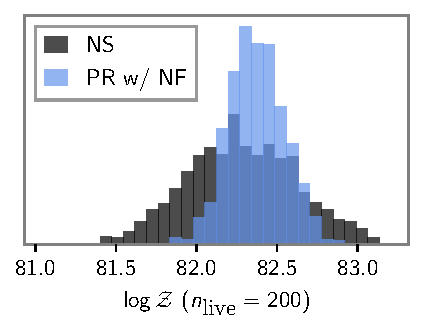
\includegraphics[]{Ca_Foscari Beamer/presentation_logZ_simulated.pdf}
    \end{figure}}
\end{minipage}

\vfill
\visible<5>{Same answer as doing a full resolution pass of NS, but \alert{7x faster} (precision-normalized).}

\end{frame}

\setbeamertemplate{headline}{
    \vspace{0.25cm} \ \ 
    
\includegraphics[height=1.0cm]{Ca_Foscari Beamer/cambridge-cropped.pdf}
    
\includegraphics[height=1.0cm]{kicc.png}
    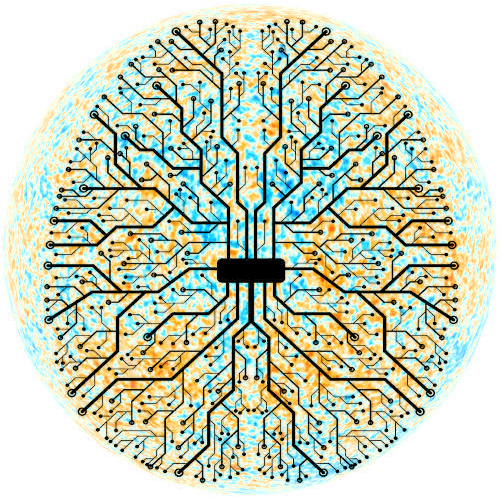
\includegraphics[height=1.0cm]{Ca_Foscari Beamer/handley-lab.png}
    \vspace{0.25cm}
    {\color{firebrick} \hrule \hrule}
  }


\setbeamertemplate{footline}{%
  \leavevmode%
  \hbox to \paperwidth{%
    % First box (Email address) - Exactly 1/3 of paperwidth
    \begingroup
    \setlength{\fboxsep}{2pt}% Padding inside the box
    \colorbox{firebrick}{\makebox[\dimexpr0.333\paperwidth\relax][c]{\strut\textcolor{white}{\texttt{myp23@cam.ac.uk}}}}%
    \endgroup
    % Second box (Custom text) - Exactly 1/3 of paperwidth
    \begingroup
    \setlength{\fboxsep}{2pt}% Padding inside the box
    \colorbox{firebrick}{\makebox[\dimexpr0.333\paperwidth\relax][c]{\strut\textcolor{white}{\href{https://openreview.net/forum?id=ekbkMSuPo4}{Yallup et al. 2025}}}}%
    \endgroup
    % Third box (Frame number) - Exactly 1/3 of paperwidth
    \begingroup
    \setlength{\fboxsep}{2pt}% Padding inside the box
    \colorbox{firebrick}{\makebox[\dimexpr0.334\paperwidth\relax][c]{\strut\textcolor{white}{\insertframenumber/\inserttotalframenumber}}}%
    \endgroup
  }%
  \vskip0pt%
}

\section{\textsc{blackjax ns}}

\setbeamertemplate{headline}{
    \vspace{0.25cm} \ \ 
    
\includegraphics[height=1.0cm]{Ca_Foscari Beamer/cambridge-cropped.pdf}
    
\includegraphics[height=1.0cm]{kicc.png}
    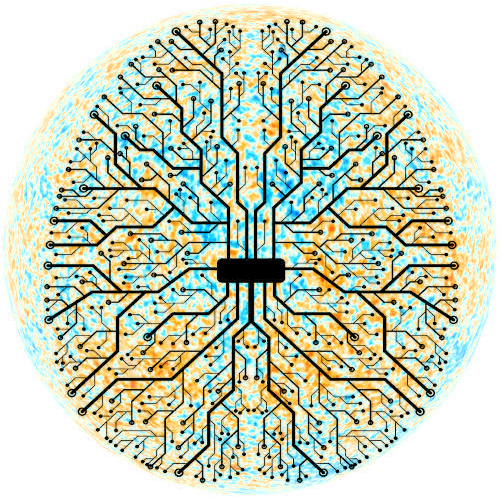
\includegraphics[height=1.0cm]{Ca_Foscari Beamer/handley-lab.png}
    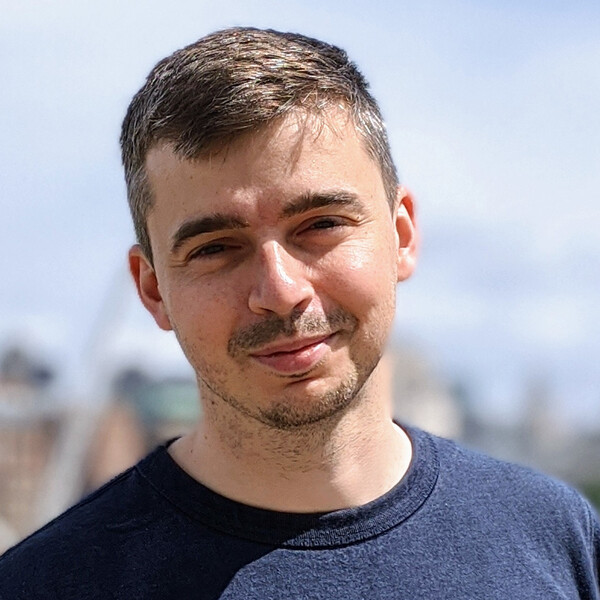
\includegraphics[height=1.0cm]{Ca_Foscari Beamer/david_yallup.jpg}
    \vspace{0.25cm}
    {\color{firebrick} \hrule \hrule}
  }

\begin{frame}{CPUs \& GPUs in Scientific Computing}
  \begin{itemize}
    \item \textbf{CPUs (Central Processing Units):}
      \begin{itemize}
        \item Optimized for a wide range of tasks.
        \item Equipped with a limited number of powerful cores.
        \item Excel at sequential, complex calculations and intricate decision-making.
        \item Ideal for tasks featuring non-uniform workloads and conditional branching.
      \end{itemize}
      \vfill
    \item \textbf{GPUs (Graphics Processing Units):}
      \begin{itemize}
        \item Architectured with thousands of smaller, efficient cores.
        \item Tailored for massive parallel arithmetic operations.
        \item Best suited for repetitive, data-parallel tasks.
        \item Increasingly used in scientific computing.
      \end{itemize}
  \end{itemize}
\end{frame}

% 1. **On the Side of CPUs:**

%    “Central Processing Units are designed for a broad range of computational tasks. They are equipped with a limited number of high-performance cores. These cores are optimized for sequential processing, complex calculations, and intricate decision-making processes. This makes CPUs particularly effective for workloads that involve non-uniform tasks and significant conditional branching.”

% 2. **On the Side of GPUs:**

%    “In contrast, Graphics Processing Units contain thousands of smaller cores that are specifically optimized for parallel arithmetic operations. This design is advantageous for repetitive tasks that can be executed concurrently across large datasets. The inherent parallelism of GPUs makes them particularly attractive in scientific computing applications, where many calculations are distributed and can be performed simultaneously.”

% 3. **Application to Gravitational Wave Inference:**

%    “Within the context of gravitational wave inference, our nested sampling algorithm benefits substantially from GPU acceleration. Many of the computational tasks, such as evaluating likelihoods across extensive parameter spaces, are naturally parallelizable. By leveraging the architecture of GPUs, we can significantly reduce computation time compared to traditional CPU implementations.”


\begin{frame}{Advantages of GPUs for GW inference}
\begin{itemize}
        \item \textbf{Likelihood Evaluation:} 
        \begin{itemize}
            \item Frequency bins are independent, so waveforms can be evaluated across many bins in parallel.
            \item On Nvidia A100 GPU, we can evaluate the waveform model $\approx O(10^9)$ times in a second for different frequencies or source parameters [\textcolor{grey}{2302.05333}].
        \end{itemize}
          
        \item \textbf{Sampling:}  
         \begin{itemize} 
         \item Multiple chains can be executed in parallel.
         \item For NS, if using a slice sampler, can run many slicing operations at once.
         \end{itemize}
      \end{itemize}
\vspace{1cm}
Parallel processing power of GPUs can speed up Bayesian inference by factor of thousands.
\end{frame}

\begin{frame}{\textsc{blackjax ns}}
    \begin{itemize}
        \item \textsc{ripple}: \textsc{jax} implementation of models for GPU-accelerated waveform calls
        \item \textsc{jim} uses \textsc{ripple} + \textsc{flowMC}
    \end{itemize}
    \vspace{1cm}
    \visible<2->{
    \bblock{\centering \textsc{blackjax NS}}
        \begin{itemize}
            \item Nested sampling implementation in \textsc{blackjax}, developed by David Yallup.
            \item 11 parameter nested sampling run on GW150914 in minutes
        \end{itemize}
    \eblock
    }
\end{frame}

\begin{frame}{Injection examples}
\vspace{2em}
    \begin{columns}
        \column{0.5\textwidth}
        %\vspace{-2em}
        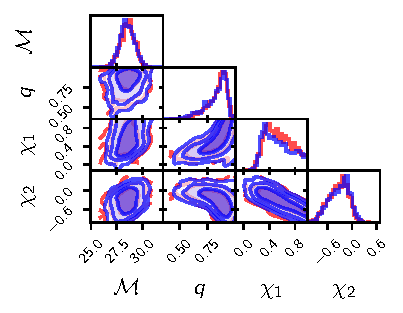
\includegraphics[]{Ca_Foscari Beamer/bilby_dynesty_blackjax_comparison_9param_intrinsic.pdf}
        \column{0.5\textwidth}
        \hspace{-3em}
        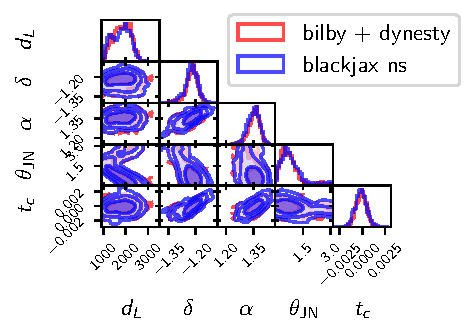
\includegraphics[]{Ca_Foscari Beamer/bilby_dynesty_blackjax_comparison_9param_extrinsic.pdf}
    \end{columns}
\end{frame}

\begin{frame}{Future of scientific computing}
  \begin{itemize}
    \item \textbf{Shift in Hardware Paradigm:}  
    \begin{itemize}
        \item  Scientific computing is increasingly relying on architectures that favor parallel operations. 
        \item Computing power will become heavily skewed towards GPUs.
    \end{itemize}
      
    \item \textbf{Implications for Research:}
      \begin{itemize}
      \item GPUs are becoming the norm in many areas, including astrophysics.
        \item Adapting our algorithms to modern hardware is essential to keep pace with the cutting edge of computing power.
      \end{itemize}
      \item \textbf{For GWs:}
      \begin{itemize}
          \item Need to get more waveforms models onto GPUs!
      \end{itemize}
  \end{itemize}
\end{frame}

\setbeamertemplate{headline}{
    \vspace{0.25cm} \ \ 
    
\includegraphics[height=1.0cm]{Ca_Foscari Beamer/cambridge-cropped.pdf}
    
\includegraphics[height=1.0cm]{kicc.png}
    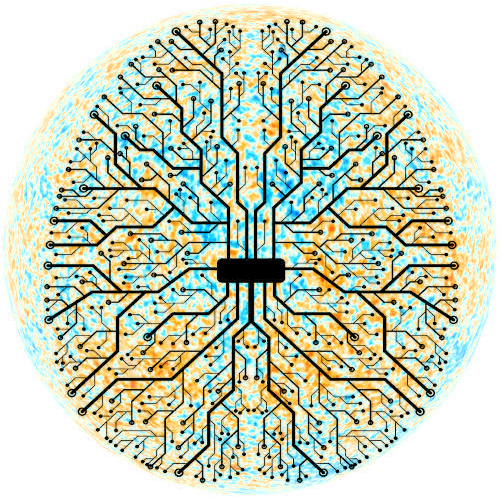
\includegraphics[height=1.0cm]{Ca_Foscari Beamer/handley-lab.png}
    \vspace{0.25cm}
    {\color{firebrick} \hrule \hrule}
  }

\begin{frame}{Conclusions}
    % Frontiers of GW PE are machine learning, SBI, GPUs. All of these are being developed in some form by the Cambridge community, meaning lots of exciting research and avenues for collaboration!
    \begin{itemize}
        \item 3G + LISA era presents significant challenges for data analysis
        \item Current standard inference methods, including traditional nested sampling, will not scale well
        \item ML-accelerated sampling and GPU-accelerated pipelines work towards addressing these challenges, and offer a complementary approach to SBI
    \end{itemize}
\end{frame}

\appendix

% reference Will for this slide
\begin{frame}{MCMC vs. NS}
    \begin{columns}
        \column{0.48\textwidth}
        \begin{block}{\textbf{MCMC}}
            % \only<16>{
            %     \begin{itemize}
            %         \item Single ``walker'', exploring posterior
            %         \item Fast, if proposal matrix is tuned
            %         \item Parameter estimation
            %     \end{itemize}
            % }
        \end{block}
            \includegraphics<1>[width=0.8\textwidth,page=16]{Ca_Foscari Beamer/himmelblau.pdf}%
            \includegraphics<2>[width=0.8\textwidth,page=17]{Ca_Foscari Beamer/himmelblau.pdf}%
            \includegraphics<3>[width=0.8\textwidth,page=18]{Ca_Foscari Beamer/himmelblau.pdf}%
            \includegraphics<4>[width=0.8\textwidth,page=19]{Ca_Foscari Beamer/himmelblau.pdf}%
            \includegraphics<5>[width=0.8\textwidth,page=20]{Ca_Foscari Beamer/himmelblau.pdf}%
            \includegraphics<6-15>[width=0.8\textwidth,page=21]{Ca_Foscari Beamer/himmelblau.pdf}%
        \centerline{\includegraphics<16>[width=0.5\textwidth,page=19]{Ca_Foscari Beamer/himmelblau.pdf}}
        \column{0.48\textwidth}
        \begin{block}<7->{\textbf{Nested sampling}}
            % \only<16>{
            %     \begin{itemize}
            %         \item Ensemble of ``live points''
            %         \item Slower than  MCMC methods
            %         \item Parameter estimation + model comparison
            %     \end{itemize}
            % }
        \end{block}
            \includegraphics<7|handout:0>[width=0.8\textwidth,page=1]{Ca_Foscari Beamer/himmelblau.pdf}%
            \includegraphics<8|handout:0>[width=0.8\textwidth,page=2]{Ca_Foscari Beamer/himmelblau.pdf}%
            \includegraphics<9|handout:0>[width=0.8\textwidth,page=3]{Ca_Foscari Beamer/himmelblau.pdf}%
            \includegraphics<10          >[width=0.8\textwidth,page=4]{Ca_Foscari Beamer/himmelblau.pdf}%
            \includegraphics<11|handout:0>[width=0.8\textwidth,page=5]{Ca_Foscari Beamer/himmelblau.pdf}%
            \includegraphics<12|handout:0>[width=0.8\textwidth,page=6]{Ca_Foscari Beamer/himmelblau.pdf}%
            \includegraphics<13|handout:0>[width=0.8\textwidth,page=7]{Ca_Foscari Beamer/himmelblau.pdf}%
            \includegraphics<14|handout:0>[width=0.8\textwidth,page=8]{Ca_Foscari Beamer/himmelblau.pdf}%
            \includegraphics<15|handout:0>[width=0.8\textwidth,page=15]{Ca_Foscari Beamer/himmelblau.pdf}%
        \centerline{\includegraphics<16>[width=0.5\textwidth,page=4]{Ca_Foscari Beamer/himmelblau.pdf}} 
    \end{columns}
\end{frame}


%---------------------------------------------------------


\end{document}
